%%% Fiktivní kapitola s instrukcemi k PDF/A

\chapter{Testování}

\section{Uživatelské testování}

Uživatelské rozhraní a celkový dojem z aplikace otestujeme pomocí rozšířené metody System Usability Scale, označované zkráceně jako SUS \citep{sus-test}. Tuto metodu představil John Brooke již v roce $1986$, stále je ale velmi aktuální, o čemž svědčí například její zmínka ve více než $1300$ publikacích.

Účastníkům testování nejprve představíme základní funkce, tedy vyhledávání receptů pomocí různých filtrů, zobrazení detailu receptu s odkazy na rozšířené informace o ingrediencích a obsah stránky s detailem ingredience. Následně jim uložíme několik úkolů, které je přimějí seznámit se s aplikací více do hloubky. Po splnění úkolů necháme uživatele vyplnit standardizovaný dotazník s $10$ otázkami a na základě odpovědí vypočteme koeficient úspěšnosti.

Výsledné skóre dotazníku se pohybuje v rozmezí od $0$ do $100$, nejedná se ale o procentuální stupnici, jak by se mohlo na první pohled zdát. Důležitá je hranice $68$ bodů --- pokud je překročena, použitelnost systému je hodnocena jako nadprůměrná. Skóre lze dále normalizovat pro přesnější interpretaci výsledků viz obrázek \ref{obr04:sus-score-system}. Nám vyšlo celkové skóre $92,5$, což lze považovat za velmi dobrý výsledek. Detaily výpočtu a~konkrétní odpovědi z~dotazníku jsou umístěny v~příloze.

\begin{figure}[h!]\centering
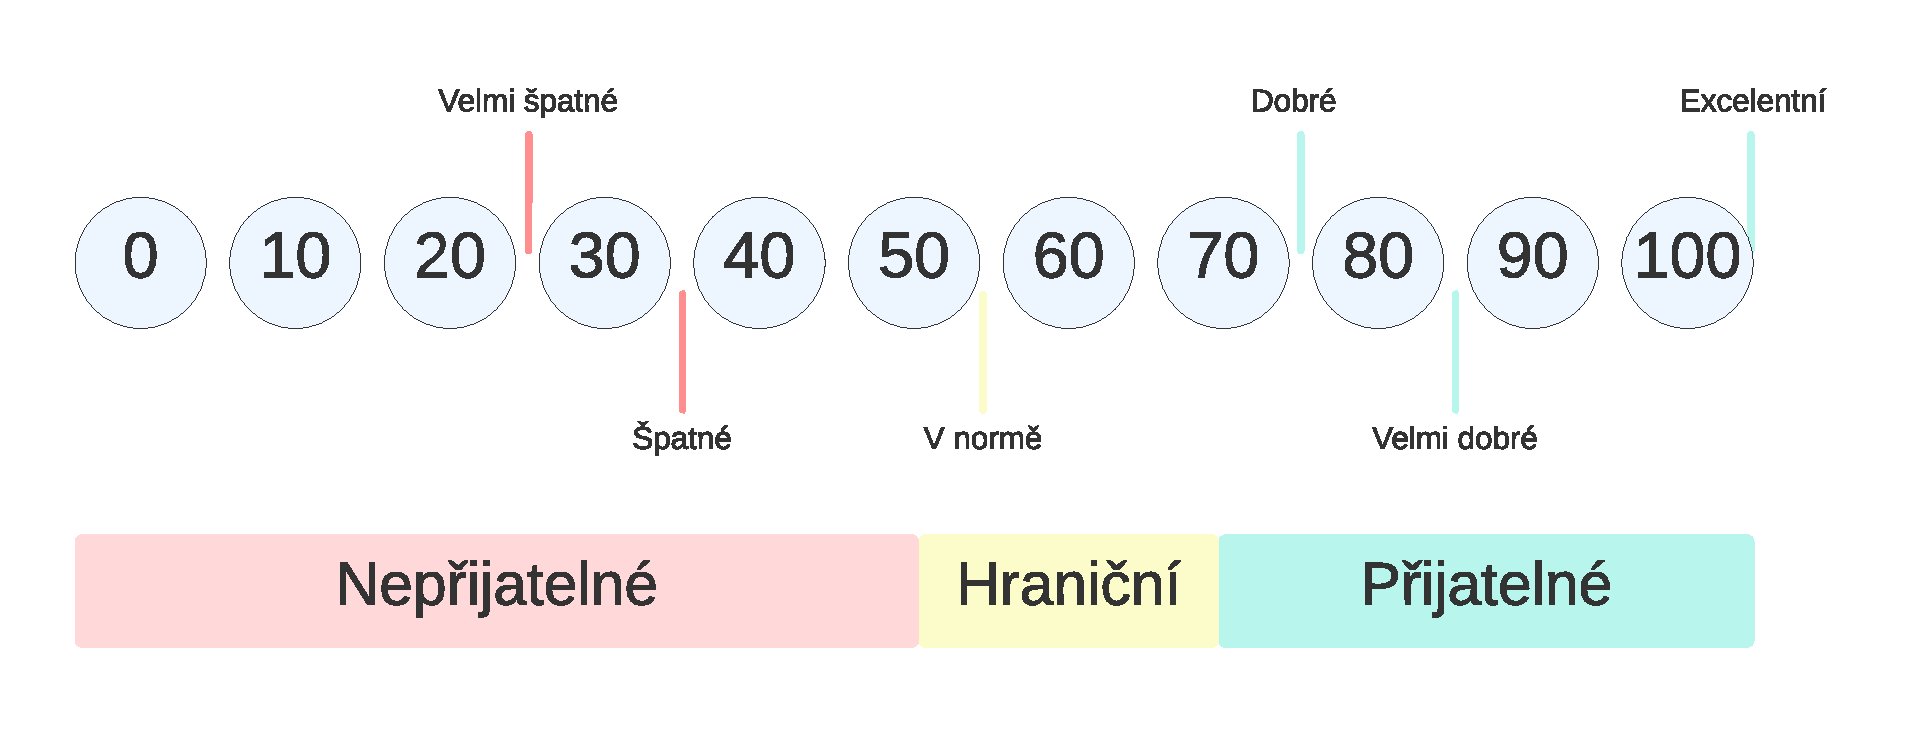
\includegraphics[width=140mm]{../img/sus-score-system}
\caption{Interpretace skóre při testování metodou System Usability Score. Adaptováno ze schématu SUS pro UX \citep{sus-adobe}.}
\label{obr04:sus-score-system}
\end{figure}

\subsection{Zadané úkoly}

Uživatelům zadáme následující úlohy, které simulují běžné využívání aplikace:

\begin{enumerate}
    \item Najděte recepty, které obsahují kuřecí prsa, rajčata a~parmazán a~je možné je připravit do $3/4$ hodiny. Poté vyhledávání změňte na recepty, které lze připravit do $1$~a~půl hodiny.
    \item Najděte nejrychlejší veganské recepty vhodné pro přípravu snídaně.
    \item Zadejte libovolné filtry a~projděte výsledky vyhledávání na první a~druhé straně. Vyberte $5$~receptů, které vás nejvíce zaujaly a~zběžně projděte jejich obsah včetně postupu přípravy.
    \item Najděte recepty z~mexické kuchyně s vysokým obsahem bílkovin a~nízkým obsahem sacharidů. Bez otevření detailů zjistěte, z~jakých ingrediencí jsou vyrobeny.
    \item Prozkoumejte ingredience na stránce vybraného receptu a~najděte suroviny ze stejných kategorií.
\end{enumerate}

\subsection{Zpětná vazba}

Nezávisle na SUS dotazníku jsme požádali testující také o~celkovou zpětnou vazbu a~nápady na vylepšení v~rámci dalšího vývoje. Celkový dojem z~používání aplikace byl pozitivní, obdrželi jsme ale řadu připomínek a~návrhů, díky kterým by práce s~aplikací byla pohodlnější a~jednodušší. Výběr nejdůležitějších z~nich, které budou vyřešeny přednostně:

\begin{enumerate}
    \item Při aktivním filtru kuchyně by se měl po kliknutí na element našeptávače zobrazit seznam ostatních kuchyní, stejně jako u~ostatních filtrů. Doprovodná zpráva \emph{No more filters} je navíc zavádějící a~sémanticky nepřesná.
    \item Při otevřeném receptu nebo ingredienci by měla být v~horní části stránky možnost navigace, aby uživatel nemusel využívat tlačítko \texttt{Zpět} ve webovém prohlížeči, které je zbytečně daleko a~ruší dojem single-page aplikace.
    \item Při návratu na vyhledávací stránku z~detailu receptu by se nemělo vyhledávání spouštět nanovo a~kurzor by se měl automaticky vrátit na poslední otevřený výsledek. Tento nedostatek byl patrný při otevírání většího počtu vyhledaných receptů.
\end{enumerate}

\subsubsection{Reakce na zpětnou vazbu}

Pro vysvětlení okolností prvního bodu, filtr kuchyně a~času přípravy se od ostatních liší tím, že lze zadat pouze jeden z~této kategorie. Našeptávač zároveň vždy ukazuje pouze ty nabídky, které generují aspoň $1$~výsledek a~zároveň menší počet výsledků, než je zobrazeno současně. 

\begin{enumerate}
    \item Zobrazení všech možností kuchyní nebo časů přípravy je problematické kvůli konceptu fasetového vyhledávání. Museli bychom vyhledávání rozdělit na $2$ požadavky, jeden včetně zadané kuchyně a~druhý bez tohoto filtru. Z~prvního požadavku bychom si vzali výsledky vyhledávání včetně připravených fasetů pro všechny filtry kromě kuchyní. Ze druhého pak speciálně jen fasetové kategorie kuchyní.
    \item Druhou připomínku můžeme snadno vyřešit pomocí komponenty známé jako \emph{breadcrumbs} v~horní části obrazovky. Hierarchie by mohla mít následující formát: \texttt{Recipes\,>\,Recipe\,Name}.
    \item Poslední zmíněná výtka se týká cachování, které jsme v~první fázi aplikace vynechali pro zjednodušení a~díky dostatečné rychlosti komunikace se Solr. Nicméně rozhodně se jedná o~důležitou funkci z~pohledu plynulosti prohlížení, je tedy v~pořadníku dalšího vývoje. Aktuálně se kurzor automaticky posouvá na první řádku výsledků při změně strany. Zvážíme také načítání pomocí nekonečného posouvání, díky kterému by uživatel nemusel přeskakovat mezi okraji stránky jako při implementaci pomocí stránkování.
\end{enumerate}

\section{Výkonnostní testování}

Zátěžové testy provedeme v~aplikaci pracující přibližně s~$91\,000$ recepty a~té\-měř $800$ ingrediencemi s~rozšiřujícími informacemi. Polovina dokumentů s~recepty pochází z~aplikace Food.com, druhá polovina z~Allrecipes. Při vyhledávání se zobrazuje maximálně $24$ výsledků na jedné straně pro optimalizaci renderování.

Všechny součásti aplikace včetně databáze CouchDB, vyhledávací platformy Solr a~serverové i~klientské části běží na jednom zařízení se stejnou IP adresou. Nemůžeme tedy zcela simulovat reálnou situaci, kdy se do zpracování vyhledávacích dotazů vloží komunikace se vzdáleným zařízením přes HTTP. Všechny API~požadavky totiž vyřizujeme lokálně.

Testovacím zařízením bude notebook Huawei se $4$-jádrovým ~procesorem Intel Core $i5$ $10$. generace a~$16$GB pamětí RAM. Na zařízení je nainstalován operační systém Windows $10$ a hlavní webové prohlížeče, na které cílíme, tedy Google Chrome, Mozilla Firefox a~Microsoft Edge. Testy výkonu provedeme pouze v prohlížeči Google Chrome, u~ostatních dvou pouze zkontrolujeme správné zobrazení aplikace. Využijeme vestavěný nástroj pro diagnostiku výkonu dostupný pod záložkou \texttt{Performance insights}. Pro účely testování vytvoříme produkční verzi aplikace pomocí příkazu \texttt{npm\,run\,build} a~následného \texttt{serve\,-s\,build}.

\subsection{Diagnostika výkonu}

Podíváme se na rychlost získávání dat ze serverové části aplikace, renderování obsahu HTML prostřednictvím modelu DOM, ale také na vizuální stabilitu jednotlivých elementů. Kromě těchto údajů diagnostika odhalila některé déle běžící funkce na hlavním vlákně. U~nich je doporučena obecná optimalizace v~podobě snížení času výpočtu na hlavním vlákně pod hranici $50\,$ms. Celkově jsou naměřené časy v~normě vzhledem k~nefunkčním požadavkům aplikace z~kapitoly o~analýze.

\subsubsection{Vyhledávání receptů}

Testy ukázaly, že obsah DOM pro obrazovku s~vyhledáváním receptů je bez zadání jakýchkoli filtrů načten průměrně za $0,5\,$s. Z toho přibližně $130\,$ms trvá získání receptů ze Solr. Vyžádáme si sice pouze $24$ receptů, chceme ale znát celkový počet pro aktuální vyhledávací dotaz. Kvůli tomu trvá zpracování dotazu na všechny recepty delší dobu než vyhledávání s~omezujícím filtrem nebo více filtry.

Z~filtrovacích dotazů jsme nejprve testovali ingredienci \texttt{Cheese}, pro kterou je k~dispozici téměř $23\,000$ receptů. Zpracování tohoto dotazu trvalo průměrně $60\,$ms, tedy o~více než polovinu kratší dobu oproti vyhledávání všech receptů. Se zadáváním dalších filtrů klesá čas potřebný pro získání dat až na průměrných $12\,$s pro dotaz filtrující právě $1$~recept. Tento klesající trend je pro naši aplikaci příznivý, neboť cílíme na specifické filtrování pomocí většího množství kritérií. Nicméně pokud bychom datovou sadu s~recepty výrazně rozšiřovali, museli bychom optimalizovat dotaz na všechny výsledky bez zadaných filtrů. Jeho zpracování by bez optimalizace trvalo příliš dlouho, což by bylo krajně nevhodné, neboť se jedná o~dotaz aktivovaný automaticky při otevření domovské stránky a~tedy první interakci uživatele s~aplikací.

\subsubsection{Detail receptu}

Získání dat receptu na základě id trvá průměrně $8\,$ms. Načtení DOM pak $0,24\,$s. Z~následného vykreslení obvykle připadne nejdelší čas (kolem $0,85\,$s) na popis receptu, pokud je text delší.

\subsubsection{Detail ingredience}

Načtení dokumentu ingredience z~backendu trvá stejně jako u~receptu přibližně $8\,$ms a~načtení DOM asi $0,3\,$s. Maximální čas vykreslení je opět spotřebován renderováním popisu (pro ingredienci \texttt{Beef} se jednalo o~$0,72\,$s).

\subsubsection{Vizuální stabilita}

Celkově by dle výsledků testování bylo potřeba zapracovat na tzv.~\emph{Cumulative Layout Shift} (CLS). Jedná se o~metriku zaměřenou na vizuální stabilitu rozložení jednotlivých elementů v HTML dokumentu. Typicky je ohrožena asynchronními požadavky, na základě kterých se data načítají postupně a~způsobují tak přeskládávání elementů. Je tedy vhodné ještě před načtením dat vytvořit aspoň základní rozložení v~očekávané velikosti, aby se následným přesunům zamezilo nebo byl zmírněn jejich dosah. Často totiž předem nevíme, v~jaké velikosti data obdržíme a~nemůžeme tak přesně odhadnout rozměry příslušného elementu. Nicméně už od skóre $0,25$ je potřeba cílit na zlepšení \citep{cls-metric} a~diagnostický nástroj u~některých z~našich elementů zachytil podstatně vyšší skóre $0,65$. Jedná se například o~sloupec s~nutričními hodnotami a~ingrediencemi na stránce detailu receptu nebo o~společnou patičku stránky.